%%%%%%%%%%%%%%%%%%%%%%%%%%%%%%%%%%%%%%%%%%%%%%%%%%%%%%%%%%%%%%%%%%%%%%%%%%%%%%%%%%%%%%%%%%%%%%%%%%%%%%%%%%%%%%%%%%%%%%%%%%%%%%%%%%%%%%%%%%%%%%%%%%%%%%%%%%%%%%%%%%%
% Written By Michael Brodskiy
% Class: Quantum Mechanics
% Professor: G. Fiete
%%%%%%%%%%%%%%%%%%%%%%%%%%%%%%%%%%%%%%%%%%%%%%%%%%%%%%%%%%%%%%%%%%%%%%%%%%%%%%%%%%%%%%%%%%%%%%%%%%%%%%%%%%%%%%%%%%%%%%%%%%%%%%%%%%%%%%%%%%%%%%%%%%%%%%%%%%%%%%%%%%%

\documentclass[12pt]{article} 
\usepackage{alphalph}
\usepackage[utf8]{inputenc}
\usepackage[russian,english]{babel}
\usepackage{titling}
\usepackage{amsmath}
\usepackage{float}
\usepackage{graphicx}
\usepackage{enumitem}
\usepackage{amssymb}
\usepackage[super]{nth}
\usepackage{everysel}
\usepackage{ragged2e}
\usepackage{geometry}
\usepackage{multicol}
\usepackage{fancyhdr}
\usepackage{cancel}
\usepackage{siunitx}
\usepackage{physics}
\usepackage{tikz}
\usepackage{mathdots}
\usepackage{yhmath}
\usepackage{cancel}
\usepackage{color}
\usepackage{array}
\usepackage{multirow}
\usepackage{gensymb}
\usepackage{tabularx}
\usepackage{extarrows}
\usepackage{booktabs}
\usepackage{lastpage}
\usetikzlibrary{fadings}
\usetikzlibrary{patterns}
\usetikzlibrary{shadows.blur}
\usetikzlibrary{shapes}

\geometry{top=1.0in,bottom=1.0in,left=1.0in,right=1.0in}
\newcommand{\subtitle}[1]{%
  \posttitle{%
    \par\end{center}
    \begin{center}\large#1\end{center}
    \vskip0.5em}%

}
\usepackage{hyperref}
\hypersetup{
colorlinks=true,
linkcolor=blue,
filecolor=magenta,      
urlcolor=blue,
citecolor=blue,
}


\title{Homework 8}
\date{\today}
\author{Michael Brodskiy\\ \small Professor: G. Fiete}

\begin{document}

\maketitle

\begin{enumerate}

  \item First and foremost, we have the wave function as:

    $$\psi_{321}(r,\theta,\phi)=-\frac{\sqrt{3}}{27\sqrt{\pi}}\sqrt[3]{\frac{Z}{3a_o}}\left( \frac{Zr}{a_o} \right)^2e^{-Zr/3a_o}\sin(\theta)\cos(\theta)e^{i\phi}$$

    We can apply the differential form $L_z$ to get:

    $$L_z\psi_{321}(r,\theta,\phi)=-i\hbar\frac{\partial}{\partial\phi}\left[\frac{\sqrt{3}}{27\sqrt{\pi}}\sqrt[3]{\frac{Z}{3a_o}}\left( \frac{Zr}{a_o} \right)^2e^{-Zr/3a_o}\sin(\theta)\cos(\theta)e^{i\phi}\right]$$
    $$L_z\psi_{321}(r,\theta,\phi)=-i\hbar\frac{\sqrt{3}}{27\sqrt{\pi}}\sqrt[3]{\frac{Z}{3a_o}}\left( \frac{Zr}{a_o} \right)^2e^{-Zr/3a_o}\sin(\theta)\cos(\theta)\frac{\partial}{\partial\phi}\left[e^{i\phi}\right]$$
    $$L_z\psi_{321}(r,\theta,\phi)=\hbar\frac{\sqrt{3}}{27\sqrt{\pi}}\sqrt[3]{\frac{Z}{3a_o}}\left( \frac{Zr}{a_o} \right)^2e^{-Zr/3a_o}\sin(\theta)\cos(\theta)e^{i\phi}$$

    We may observe that this gives us $L_z\psi_{321}=\hbar\psi_{321}$, and, therefore, $\psi_{321}$ is an eigenstate of $L_z$ with eigenvalue $\hbar$ (as expected with $m=1$). We now proceed to check $\vec{L}^2$:

    $$\vec{L}^2\psi_{321}(r,\theta,\phi)=-\hbar^2\left[\frac{1}{\sin(\theta)}\frac{\partial}{\partial\theta}\left( \sin(\theta)\frac{\partial}{\partial\theta} \right)+\frac{1}{\sin^2(\theta)}\frac{\partial^2}{\partial\phi^2}\right]\psi_{321}(r,\theta,\phi)$$

    We pull out $r$-dependent terms as constants (let us express these as $\bold{R}$), which gives us:

    $$\vec{L}^2\psi_{321}(r,\theta,\phi)=-\hbar^2R\left[ \frac{1}{\sin(\theta)}\frac{\partial}{\partial\theta}\left[ \sin(\theta)\frac{\partial}{\partial\theta} \sin(\theta)\cos(\theta) \right]e^{i\phi} +\cot(\theta)\frac{\partial^2}{\partial\phi^2} e^{i\phi}\right]$$
    $$\vec{L}^2\psi_{321}(r,\theta,\phi)=-\hbar^2Re^{i\phi}\left[ \frac{1}{\sin(\theta)}\frac{\partial}{\partial\theta}\left[ \sin(\theta)\cos^2(\theta)-\sin^3(\theta) \right]-\cot(\theta)\right]$$
    $$\vec{L}^2\psi_{321}(r,\theta,\phi)=-\hbar^2Re^{i\phi}\left[ \frac{1}{\sin(\theta)}\left[ \cos^3(\theta)-5\cos(\theta)\sin^2(\theta) \right]-\cot(\theta)\right]$$
    $$\vec{L}^2\psi_{321}(r,\theta,\phi)=-\hbar^2Re^{i\phi}\left[ \cos^2(\theta)\cot(\theta)-5\cos(\theta)\sin(\theta)-\cot(\theta)\right]$$

    Using trigonometric identities, we may simplify to:

    $$\vec{L}^2\psi_{321}(r,\theta,\phi)=-\hbar^2Re^{i\phi}\left[ -6\cos(\theta)\sin(\theta)\right]$$

    And finally:

    $$\vec{L}^2\psi_{321}(r,\theta,\phi)=6\hbar^2Re^{i\phi}\left[ \cos(\theta)\sin(\theta)\right]$$
    
    We may see that this indicates that $\psi_{321}$ is, indeed, an eigenfunction of $\vec{L}^2$, with eigenvalue $6\hbar^2$ (which would be expected for $l=2$, since $[2(2+1)]$ gives us $6$). Finally, we check the Hamiltonian, which can be expressed as:

    $$H=-\frac{\hbar^2}{2\mu}\left[ \frac{1}{r^2}\frac{\partial}{\partial r}\left( r^2\frac{\partial}{\partial r} \right)+\frac{1}{r^2\sin(\theta)}\frac{\partial}{\partial \theta}\left( \sin(\theta)\frac{\partial}{\partial\theta}+\frac{1}{r^2\sin(\theta)}\frac{\partial^2}{\partial\phi^2} \right) \right] + V(r)$$

    Before we evaluate, we can simplify this to:

    $$H=-\frac{\hbar^2}{2\mu}\left[ \frac{1}{r^2}\frac{\partial}{\partial r}\left( r^2\frac{\partial}{\partial r}\right) -\frac{\vec{L}^2}{r^2\hbar^2}\right]-\frac{Ze^2}{4\pi\varepsilon_or}$$

    We take $\mu\to m_e$ to give us:

    $$H\psi_{321}=-\frac{\hbar^2}{2m}\left[ \frac{1}{r^2}\frac{\partial}{\partial r}\left( r^2\frac{\partial}{\partial r}\right) -\frac{\vec{L}^2}{r^2\hbar^2}-\frac{2mZe^2}{4\pi\varepsilon_or\hbar^2}\right]\psi_{321}$$

    From here, we proceed to evaluate (note, we simplify the $\theta$ and $\phi$ dependent terms as $\Theta$ and $\Phi$):

    $$H\psi_{321}=-\frac{\hbar^2}{2m}\left[ \sqrt{\frac{1}{3\pi}}\left( \frac{Z}{3a_o} \right)^{7/2}\right]\left[ \frac{1}{r^2}\frac{\partial}{\partial r}\left( 2r^3-\frac{Zr^4}{3a_o} \right)-\left( \frac{6}{r^2}-\frac{mZe^2}{2\pi\varepsilon_or\hbar^2} \right)r^2 \right]e^{-Zr/3a_o}\Theta\Phi$$
    $$H\psi_{321}=-\frac{\hbar^2}{2m}\left[ \sqrt{\frac{1}{3\pi}}\left( \frac{Z}{3a_o} \right)^{7/2}\right]\left[ \left( 6-\frac{2Zr}{a_o}+\frac{Z^2r^2}{9a_o^2} \right)-6+\frac{mZe^2r}{2\pi\varepsilon_o\hbar^2} \right]e^{-Zr/3a_o}\Theta\Phi$$
    $$H\psi_{321}=-\frac{\hbar^2}{2m}\left[ \sqrt{\frac{1}{3\pi}}\left( \frac{Z}{3a_o} \right)^{7/2}\right]\left[ \frac{Z^2r^2}{9a_o^2} \right]e^{-Zr/3a_o}\Theta\Phi$$
    $$H\psi_{321}=-\frac{1}{9}\frac{\hbar^2Z^2}{2ma_o^2}\psi_{321}$$
    $$\boxed{H\psi_{321}=-\frac{Z^2}{9}\text{Ryd}\psi_{321}}$$

   Thus, we see that the energy eigenvalue is $-Z^2\text{Ryd}/9$, as would make sense for $n=3$.

  \item

    \begin{enumerate}

      \item First and foremost, we see that, for this superposition state, the possible energies are given by the $n$ values, or $n=2,3,4$:

        $$\boxed{E_2=-\frac{13.6}{4}=-3.4[\si{eV}]}$$
        $$\boxed{E_3=-\frac{13.6}{9}=-1.511[\si{eV}]}$$
        $$\boxed{E_4=-\frac{13.6}{16}=-.85[\si{eV}]}$$

        The probabilities will be given by the squares of the magnitudes of the coefficients such that:

        $$\boxed{P_{E_2}=\left( \frac{1}{\sqrt{14}} \right)^2=\frac{1}{14}}$$
        $$\boxed{P_{E_3}=\left( \frac{-2}{\sqrt{14}} \right)^2=\frac{2}{7}}$$
        $$\boxed{P_{E_4}=\left( \Big|\frac{3i}{\sqrt{14}}\Big| \right)^2=\frac{9}{14}}$$

        Thus, we obtain the following histogram:

        \begin{figure}[H]
          \centering
          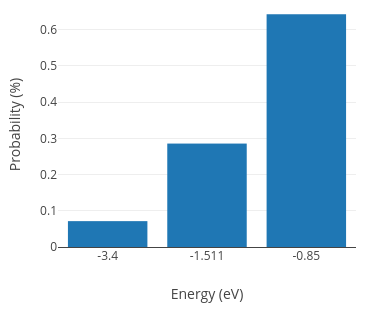
\includegraphics[width=.5\textwidth]{Figures/HW8-2a}
          \caption{Histogram of Energy Probabilities}
          \label{fig:1}
        \end{figure}

        We proceed to calculate the expectation value of energy as:

        $$\langle E\rangle =\bra{\psi|H}\ket{\psi}$$
        $$\bra{\psi|H}\ket{\psi}=-13.6\sum_{n=1}^{\infty} \frac{P_{E_n}}{n^2}$$
        $$-13.6\sum_{n=1}^{\infty} \frac{P_{E_n}}{n^2}=-13.6\left( \frac{1/14}{4}+\frac{4/14}{9}+\frac{9/14}{16} \right)$$
        $$\boxed{\langle E\rangle=-1.221[\si{eV}]}$$

      \item We know that $\vec{L}^2$ is limited to $l(l+1)\hbar^2$, and that $l$ is limited by the superimposed states. Accordingly, we may find that the possible measurements are $\boxed{\vec{L}^2=2\hbar^2,6\hbar^2}$. The probabilities can then be calculated as:

        $$\boxed{P_{l=1}=\left( \frac{1}{\sqrt{14}} \right)^2=\frac{1}{14}}$$
        $$\boxed{P_{l=2}=\left( \frac{-2}{\sqrt{14}} \right)^2+\Big|\frac{3i}{\sqrt{14}}\Big|^2=\frac{13}{14}}$$

        Accordingly, we may plot the histogram as:

        \begin{figure}[H]
          \centering
          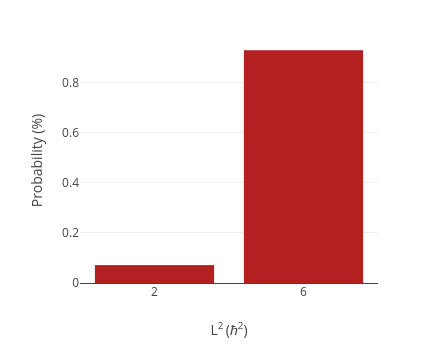
\includegraphics[width=.5\textwidth]{Figures/HW8-2b}
          \caption{Histogram of Spin Vector Probabilities}
          \label{fig:2}
        \end{figure}

        We calculate the expectation value in a manner similar to part (a) to get:

        $$\langle \vec{L^2}\rangle=\hbar^2\left( \frac{2}{14}+\frac{6(13)}{14} \right)$$
        $$\boxed{\langle \vec{L^2}\rangle=5.7143\hbar^2}$$

      \item By the eigenvalues, we know that $L_z$ can be $m\hbar$. As such, we see that $m=1,-1,2$, which gives us measurements of $\pm\hbar,2\hbar$. We can then find the probabilities as:

        $$\boxed{P_{-\hbar}=\left( \frac{-2}{\sqrt{14}} \right)^2=\frac{2}{7}}$$
        $$\boxed{P_{\hbar}=\left( \frac{1}{\sqrt{14}} \right)^2=\frac{1}{14}}$$
        $$\boxed{P_{-\hbar}=\left( \Big|\frac{3i}{\sqrt{14}} \Big|\right)^2=\frac{9}{14}}$$

        We can then plot the histogram as:

        \begin{figure}[H]
          \centering
          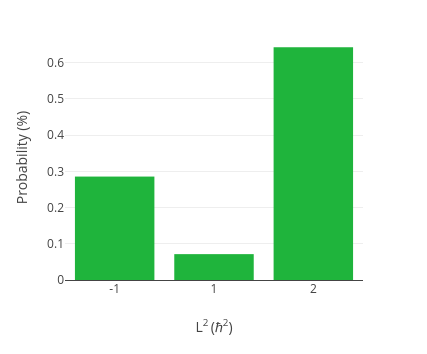
\includegraphics[width=.5\textwidth]{Figures/HW8-2c}
          \caption{Histogram of $L_z$ Probabilities}
          \label{fig:3}
        \end{figure}

        Finally, we calculate the expectation value as:

        $$\langle L_z\rangle = \frac{-4\hbar}{14}+\frac{\hbar}{14}+\frac{18\hbar}{14}$$
        $$\boxed{\langle L_z\rangle = \frac{15\hbar}{14}}$$

      \item We may observe that the answers to (a), (b), and (c) are not dependent on time (\textit{i}.\textit{e}.\ they are stationary quantities) since the operators commute with the Hamiltonian

    \end{enumerate}

\end{enumerate}

\end{document}

